\documentclass[11pt,letter]{moderncv}

\moderncvtheme[grey]{casual}

\usepackage[margin=1in]{geometry}

\usepackage{background}

\usepackage{tkz-graph}
\usetikzlibrary{arrows,shapes,decorations.markings}

\tikzstyle{every picture}+=[
  xnode/.style={fill=gray!20,shape=rectangle,draw},
  ynode/.style={fill=white!100,shape=circle,draw},
  enode/.style={fill=white!100,shape=rectangle,draw}
]

\newcommand*{\cyccwl}[2][.5cm]{\draw[decoration={markings, mark=at position .5 with {\arrowreversed{triangle 90}}}, postaction={decorate}] #2 circle (#1)}

\newcommand*{\cycccwl}[2][.5cm]{\draw[decoration={markings, mark=at position .5 with {\arrow{triangle 90}}}, postaction={decorate}] #2 circle (#1)}

\newcommand*{\cyccwr}[2][.5cm]{\draw[decoration={markings, mark=at position 0 with {\arrowreversed{triangle 90}}}, postaction={decorate}] #2 circle (#1)}

\newcommand*{\cycccwr}[2][.5cm]{\draw[decoration={markings, mark=at position 0 with {\arrow{triangle 90}}}, postaction={decorate}] #2 circle (#1)}

\backgroundsetup{
  color=black!12,
  scale=4,
  angle=-47,
  hshift=-15,
  vshift=-7,
  contents={
    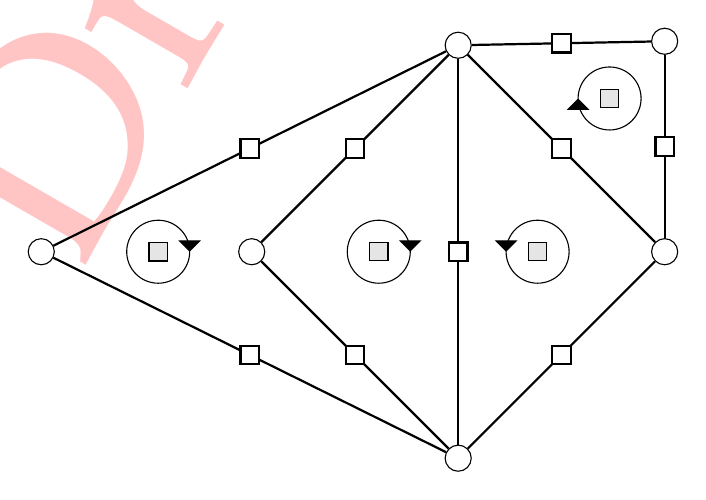
\begin{tikzpicture}
      \def\nodesep{2.5cm}
      \def\cycrad{0.4cm}
      \node[style=ynode] (a) at (0, 0) {};
      \node[style=ynode,above left = \nodesep] at (a) (d) {};
      \node[style=ynode,above right = \nodesep] at (a) (f) {};
      \node[style=ynode,above right = \nodesep] at (d) (c) {};
      \node[style=ynode,left = \nodesep] at (d) (b) {};
      \node[style=ynode,above = \nodesep] at (f) (e) {};
      %
      \path [draw, thick] (a) to node[style=enode] (4) {} (c);
      \path [draw, thick] (a) to node[style=enode] (9) {} (f);
      \path [draw, thick] (a) to node[style=enode] (2) {} (d);
      \path [draw, thick] (a) to node[style=enode] (1) {} (b);
      \path [draw, thick] (b) to node[style=enode] (6) {} (c);
      \path [draw, thick] (d) to node[style=enode] (5) {} (c);
      \path [draw, thick] (f) to node[style=enode] (3) {} (c);
      \path [draw, thick] (c) to node[style=enode] (8) {} (e);
      \path [draw, thick] (f) to node[style=enode] (7) {} (e);
      %
      \node [style=xnode] (A) at (barycentric cs:f=1,c=1,e=1.75) {};
      \node [style=xnode] (B) at (barycentric cs:a=1,d=1.25,c=1) {};
      \node [style=xnode] (C) at (barycentric cs:a=1,c=1,f=1.25) {};
      \node [style=xnode] (D) at (barycentric cs:b=1,d=1.25) {};
      %
      \cyccwl[\cycrad]{(A)};
      \cyccwr[\cycrad]{(B)};
      \cycccwl[\cycrad]{(C)};
      \cyccwr[\cycrad]{(D)};
      %
    \end{tikzpicture}
  }
}

\usepackage{mathpazo}
\renewcommand{\sfdefault}{\rmdefault}

\firstname{Andrew}
\familyname{Gainer-Dewar}
\address{510 Fourth Street East}{Northfield, MN 55057}
\mobile{(617) 444-9974}
\email{gainer.andrew@gmail.com}

\begin{document}
\maketitle

\section{Experience}
\cventry{Fall 2012 -- Spring 2013}{Visiting Assistant Professor of Mathematics}{Carleton College}{Northfield}{MN}{
  \begin{itemize}
  \item Will teach five total sections of first- and second-semester calculus and linear algebra
  \item Supervising small group senior research (`comps') project in graph enumeration
  \end{itemize}
}

\cventry{Fall 2008 -- Spring 2010}{Graduate teaching fellow}{Brandeis University}{Waltham}{MA}{Taught sections of precalculus, first- and second-semester calculus, and linear algebra}

\cventry{2008 -- 2009}{\LaTeX{} proofreader}{Harvard University Accessible Technologies Lab}{Cambridge}{MA}{Proofread \LaTeX{} versions of scanned course materials for blind physics Ph.D.\ student}

\cventry{various}{Mathematics grader}{Mercer and Brandeis}{}{}{}

\cventry{various}{Mathematics and writing tutor}{Mercer and Brandeis}{}{}{}

\section{Education}
\cventry{2007--2012}{Ph.D.\ (Mathematics)}{Brandeis University}{Waltham}{MA}{Supervisor: Ira Gessel}

\cventry{2003--2007}{B.S.\ (Mathematics) \& B.A.\ (Philosophy)}{Mercer University}{Macon}{GA}{`Outstanding Senior' awards from both depts., \textit{magna cum laude}, University Honors}

\cventry{Summer 2005}{REU}{Valparaiso University}{Valparaiso}{IN}{NSF-sponsored REU, researched crystallographic groups}

%Publications section (header added by \bibliography)
\nocite{*}
\bibliographystyle{publist/utphys}
\bibliography{publist/publist}

\section{Undergraduate research supervised}
\cventry{Fall--Winter 2012}{On the species of bipartite point-determining graphs}{Carleton College}{Northfield}{MN}{
  Supervising four senior math majors in capstone project\\
  Students are studying species theory and will apply it to open enumeration problems concerning bipartite graphs and $(k,l)$-trees
}

\clearpage

\section{Presentations and talks}
\cventry{January 2013}{$\Gamma$-species and the enumeration of \boldmath{$k$}-trees}{}{}{}{
  Short overview of results in paper of same title\\
  Joint Mathematics Meetings, San Diego
}

\cventry{Spring 2012}{Contemporary graph enumeration and \boldmath{$k$}-trees}{}{}{}{
  Defense of Ph.D.\ dissertation
}

\cventry{Spring 2012}{Arrow's Theorem and the impossibility of democracy}{}{}{}{
  Non-technical introduction to social choice and voting theory\\
  Brandeis Graduate Student Seminar, Carleton College
}

\cventry{Fall 2011}{Categorial combinatorics and the theory of species}{}{}{}{
  Survey of species theory, Brandeis GSS
}

\cventry{Spring 2007}{Piecewise-linear boundaries of surfaces that immerse isometrically in $\mathbf{R}^2$}{}{}{}{
  Won JMM Undergraduate Poster Session prize
}

\section{Service}
\cventry{January 2013}{JMM Undergraduate Poster Session Judge}{}{}{}{}
\cventry{2012--}{Department social co-coordinator}{Carleton}{}{}{}
\cventry{2012--}{Math GRE preparation co-coordinator}{Carleton}{}{}{}
\cventry{2008--2012}{Graduate student representative}{Brandeis}{}{}{
  \begin{itemize}
  \item Coordinated department graduate student seminar, semiannual barbecues, and weekly tea
  \item Represented graduate students in departmental decision-making including funds allocation and graduate teaching requirements
  \end{itemize}
}
\end{document}
